%=====================%
\chapter{Simulation}
%=====================%
%-------------------------------------------------------------------%
\section{Geant Simulation}
%-------------------------------------------------------------------%

Using Geant4 [18], we have created a replica of the APEX geometry for our simulation. Most of the code
for the detector construction was written by Stephen Daigle. Some improvements have recently been made
by an undergraduate, Chiara Salemi, who is working with our group. We have added additional components
to the simulation, specically the electromagnet and a holder containing the source and aerogel. I have
implemented one possible source holder in the simulation (Figure 11), complete with the positron source
(22Na) deposited on kapton foil and sandwiched between pieces of scintillator and aerogel. In the simulation,
as in the physical world, a positron exiting the source is tagged and then scatters within the aerogel until
it loses enough kinetic energy to form positronium. The aluminium source and all of its constituents were
incorporated into the simulation this past year.


%-------------------------------------------------------------------%
\section{Another Section}
\label{sec:mjd}
%-------------------------------------------------------------------%
 \section{Experimental Setup}

\subsection{Positronium Formation, Decay, and Detection}

Our experiment can be conceptualized by visualizing the trajectory of a positron which originates in the center of the array and mentally tracking its subsequent interactions. The positron is emitted from a $\mathrm{{}^{22}Na}$ source in the middle of our detector. $\mathrm{{}^{22}Na}$ decays via the emission of a beta particle (Figure 10) to an excited state of $\mathrm{{}^{22}Ne}$, with a $90\%$ branching ratio. This state is short-lived and decays to the ground state of the $\mathrm{{}^{22}Ne}$ via emission of a 1.274 MeV gamma ray. Because the lifetime of the excited state is so short, the 1.274 MeV gamma ray can be used in the event selection process. 

Figure 5 shows a schematic of the proposed experiment. The $\mathrm{{}^{22}{Na}}$ is deposited on two thin sheets of kapton foil and sandwiched between scintillator. The scintillator, which is orthogonal to the $z$-axis of our cylindrical detector, tags the positron as it leaves the source. An optical fiber fed through a small hole in the source holder propagates the scintillation light to a nearby photomultiplier tube. This is the ``start signal'' for an event. The entire source holder is designed to be suspended in the center of the experiment via two long, hollow rods which fit into bore holes in the electromagnet.

Still in the source holder, the positron exits the scintillator and into an adjacent disk of aerogel. Aerogel is comprised of silica dioxide chains folded in such a way that the resulting material is highly porous. The aerogel borders the scintillator on both sides. Once the positron loses nearly all of its energy via scattering, it interacts with an electron in the $\mathrm{SiO_{2}}$ to form positronium. The positronium travels almost freely in the interstitial spaces of the aerogel until it decays, minimizing matter-interaction effects. The average lifetime of the $m=0$ states of positronium ($\sim$22 ns) is dictated by the 5 kGauss (0.5 T) magnetic field generated by our C-shaped electromagnet. We selected this field strength based on the optimum fields determined by previous groups. We will likely adjust this field strength as our studies of systematics mature. The electromagnet serves the dual purpose of separating our the spin states of ortho-positronium and providing spin-alignment. Based on the modeling described below, we have determined that our field inhomogeneity will be less than $2\%$, a significant improvement over the $10\%$ inhomogeneity of past experiments. Furthermore, we have the ability to switch the magnet's polarity, which will further reduce our systematics. This improvement has been suggested but not implemented by those who worked on previous $CP$-violating searches in positronium. The magnet is tapered in such a way that it cannot interfere with the trajectory of any positronium gamma ray which could be counted in our detector.

Gamma rays from the positronium decay propagate outwards, leaving the source holder and eventually reaching the sodium iodide segments of our detector, where they interact via the photoelectric effect and compton scattering. We use the APEX (ATLAS Positron Experiment~\cite{Mercer1994491}) array, a detector which consists of 24 trapezoidal sodium iodide segments (Figure 6). The dimensions of each segment is $\mathrm{55{\times}6{\times}5.5(7.0)\,cm^3}$. Each sodium iodide bar is bookended by two photomultiplier tubes, which pick up the resulting scintillation light in the crystal. The photomultiplier tubes run to the DAQ, situated in an electronics rack. Both the APEX detector and the electronics already exist at TUNL. 

 The cross section of the experiment is shown below.
 \begin{figure}[H]
 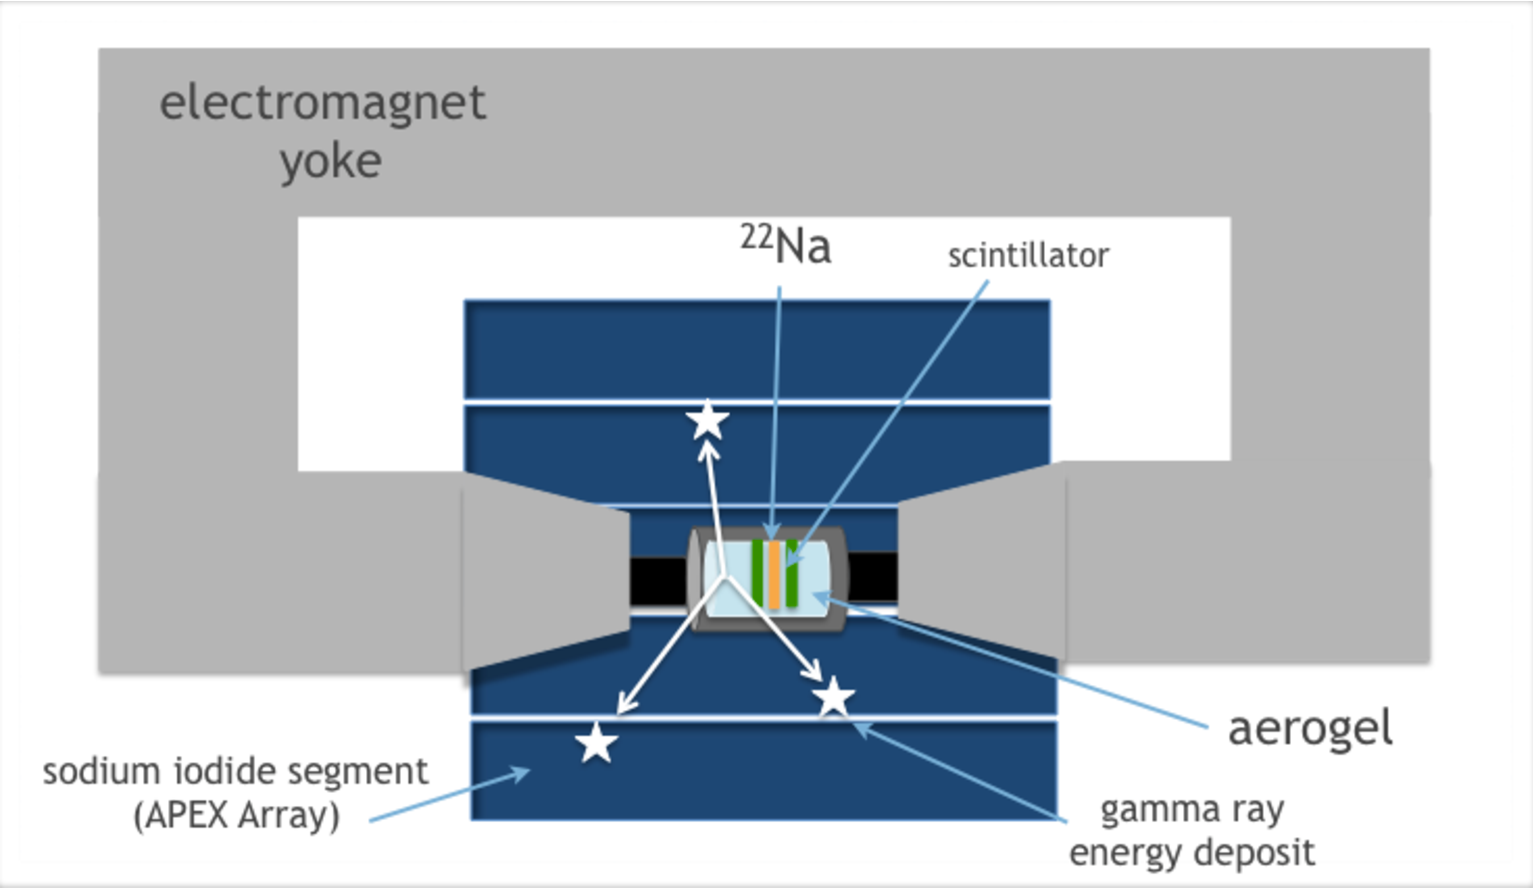
\includegraphics[width=0.75\textwidth,center]{CALIOPE_CrossSec.pdf}
 \caption{CALIOPE Cross Section (Bird's Eye View)}
 \end{figure}


\begin{wrapfigure}{r}{0.34\textwidth}
 \vspace{-10pt}
  \begin{center}
    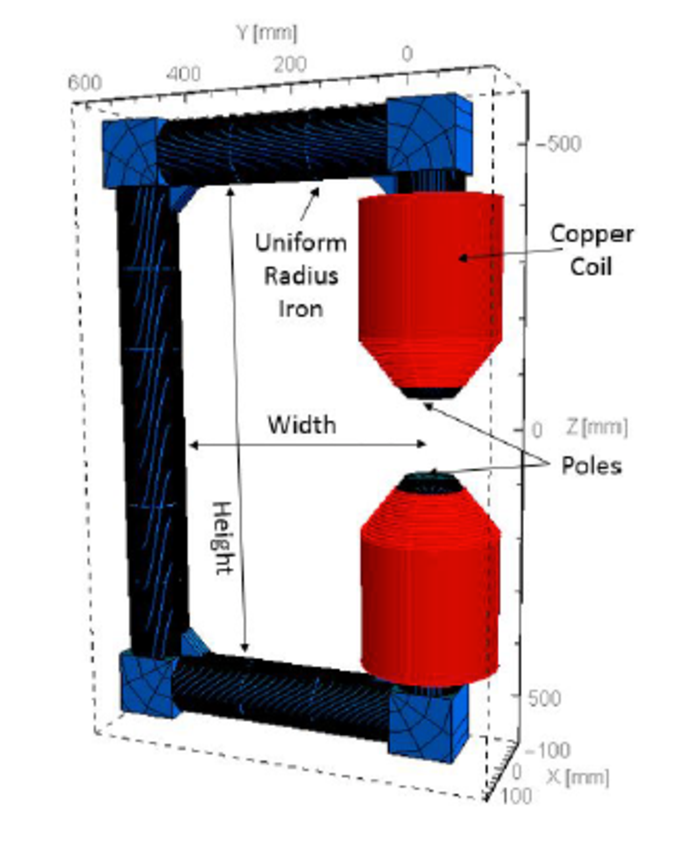
\includegraphics[width=0.34\textwidth]{Magnet.pdf}
  \end{center}
 \vspace{-10pt}
  \caption{Magnet}
\end{wrapfigure}

\subsection{Event Reconstruction}
 We calculate the position and energy of the hits in our detector by using the charge amplitudes measured by the photomultiplier tubes and a technique developed by a former graduate student, Stephen Daigle~\cite{StephenDaigle}. The amplitude of the signal from the first photomultiplier tube is
 \begin{align}
   A_{1}=\frac{E_{\gamma}P}{E_{0}}\exp[-\mu(L/2+z)]
 \end{align}
 where $z$ is the position of a hit, $E_{\gamma}$ is the energy deposited by the gamma ray, $P$ is the quantum efficiency of the photomultiplier tubes, $E_{0}$ is the energy deposited per light photon created in the scintillator and $\mu$ is the light attenuation coefficient. The attenuation coefficients were all measured by Stephen Daigle~\cite{StephenDaigle}. For the second photomultiplier tube, we have a similar equation:
 \begin{align}
 A_{2}=\frac{E_{\gamma}P}{E_{0}}\exp[-\mu(L/2-z)]
 \end{align}
 We can combine these equations to find the position in the bar from the charge amplitudes.
\begin{align}
 &z=\frac{1}{2\mu}\ln\frac{A_{2}}{A_{1}}
 \end{align}
 The resolution for the $z$ position was measured to be 3.5 cm FWHM.
 In a similar manner, the energy can also be calculated from the charge amplitudes using the following equation:
 \begin{align}
 &{E_{\gamma}}^{2}=A_{1}A_{2}\left(\frac{E_{0}}{P}\right)^2e^{{\mu}L} \\
 &E_{\gamma}=\sqrt{A_{1}A_{2}}\frac{E_{0}}{P}e^{{\mu}L/2}
 \end{align}

%\begingroup
%\setlength{\intextsep}{3pt}%
%\setlength{\columnsep}{3pt}%
% \begin{wrapfigure}{l}{0.32\textwidth}
% \vspace{-10pt}
%   \begin{center}
 %    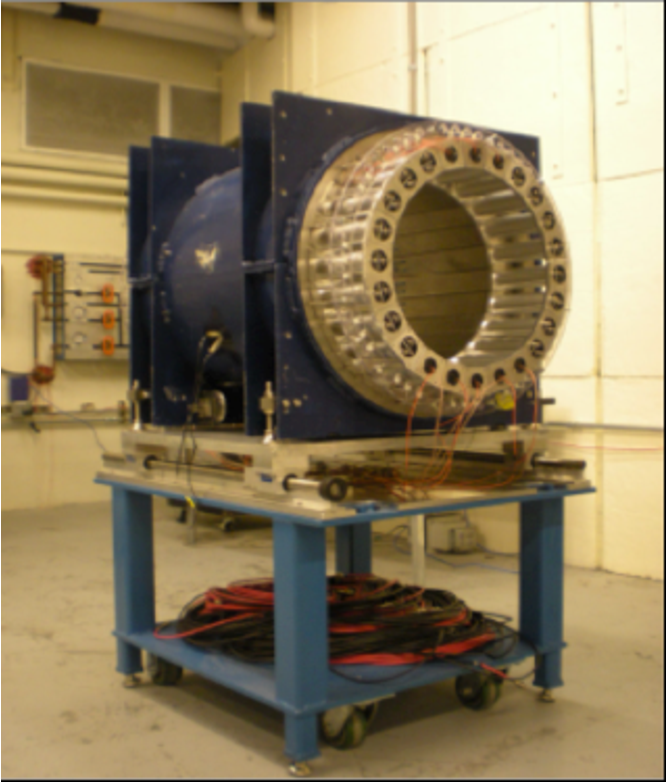
\includegraphics[width=0.32\textwidth]{APEX_Array.pdf}
 %  \end{center}
 %\vspace{-10pt}
 %  \caption{APEX Array at TUNL}
 %\end{wrapfigure}
%\endgroup


 \begin{figure}[!htb]
     \centering
     \begin{minipage}{.5\textwidth}
         \centering
         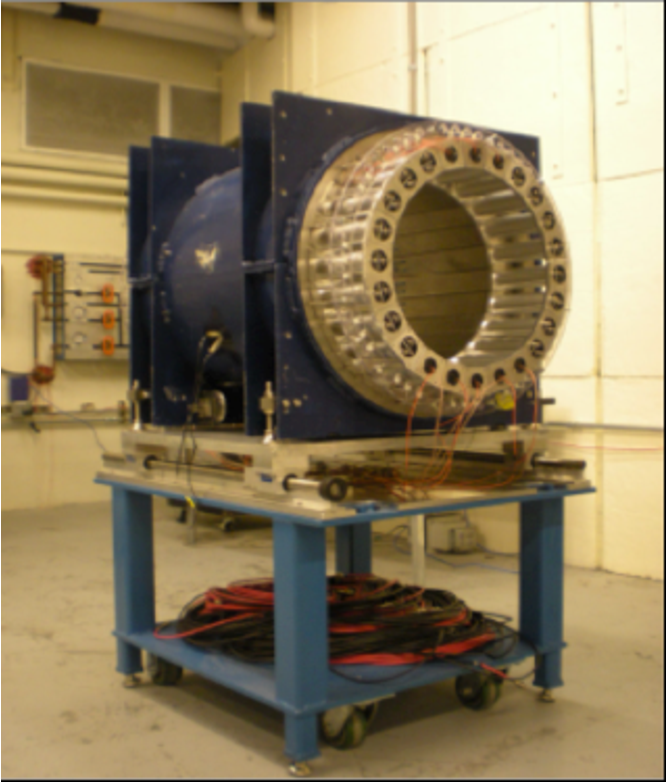
\includegraphics[width=0.6\linewidth]{APEX_Array.pdf}
         \caption{Side View of APEX at TUNL}
     \end{minipage}%                                                                                                                                                     
     \begin{minipage}{0.5\textwidth}
       \centering
       \includegraphics[width=0.7\linewidth]{APEX_Center.pdf}
       \caption{Front View of APEX at TUNL}
     \end{minipage}
 \end{figure}

 The resolution for the energy was measured to be 15\% for the 662 keV gamma ray line in $\mathrm{{}^{137}{Cs}}$. The large solid-angle coverage (75\%) and high intrinsic efficiency result in a total photopeak detection probability of 17\% at 1332 keV, as measured by Perry et al~\cite{2003NIMPA.505...85P}. 

 \begin{figure}[H]
 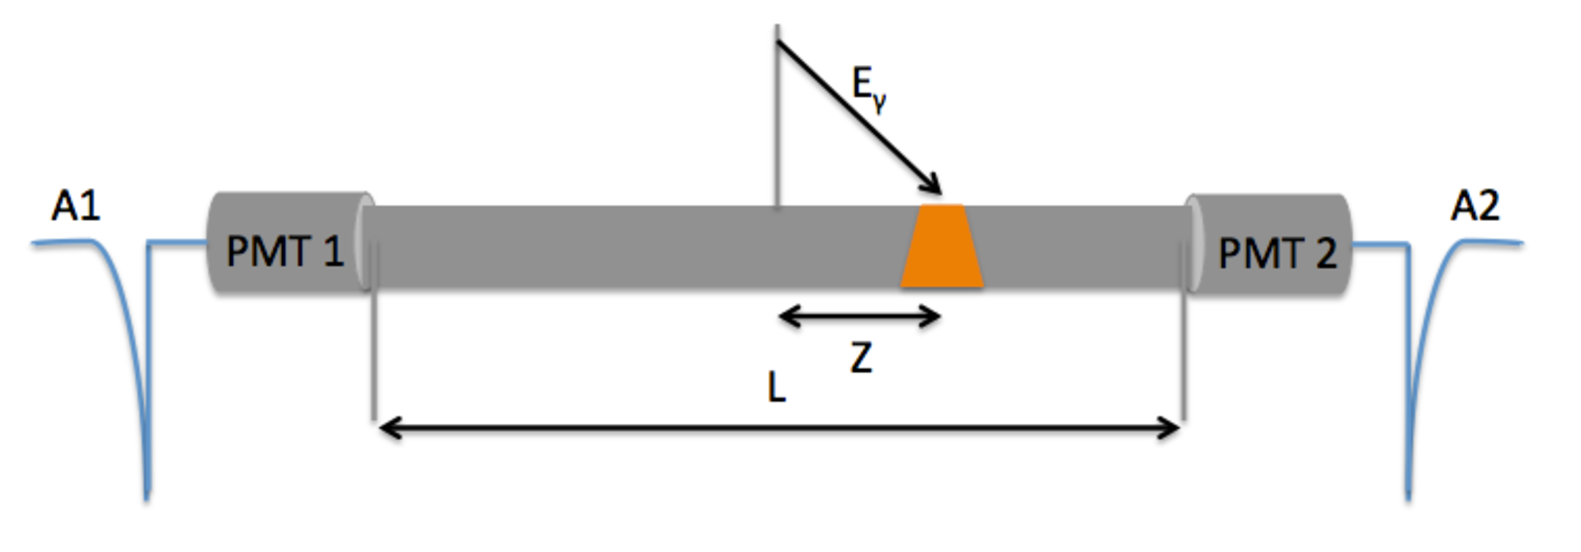
\includegraphics[width=0.7\textwidth,center]{NaI_Bar.pdf}
 \caption{NaI Segment}
 \end{figure}

This concludes our overview of the CALIOPE experiment. In the following section, we once again work from the inside out to present our experimental progress. We describe all facets of the construction, from the design phase up to the commissioning and integration of all major components of the experiment.


% ------------  figure start  
% from M. Busch
\begin{figure}[htbp]
\centering
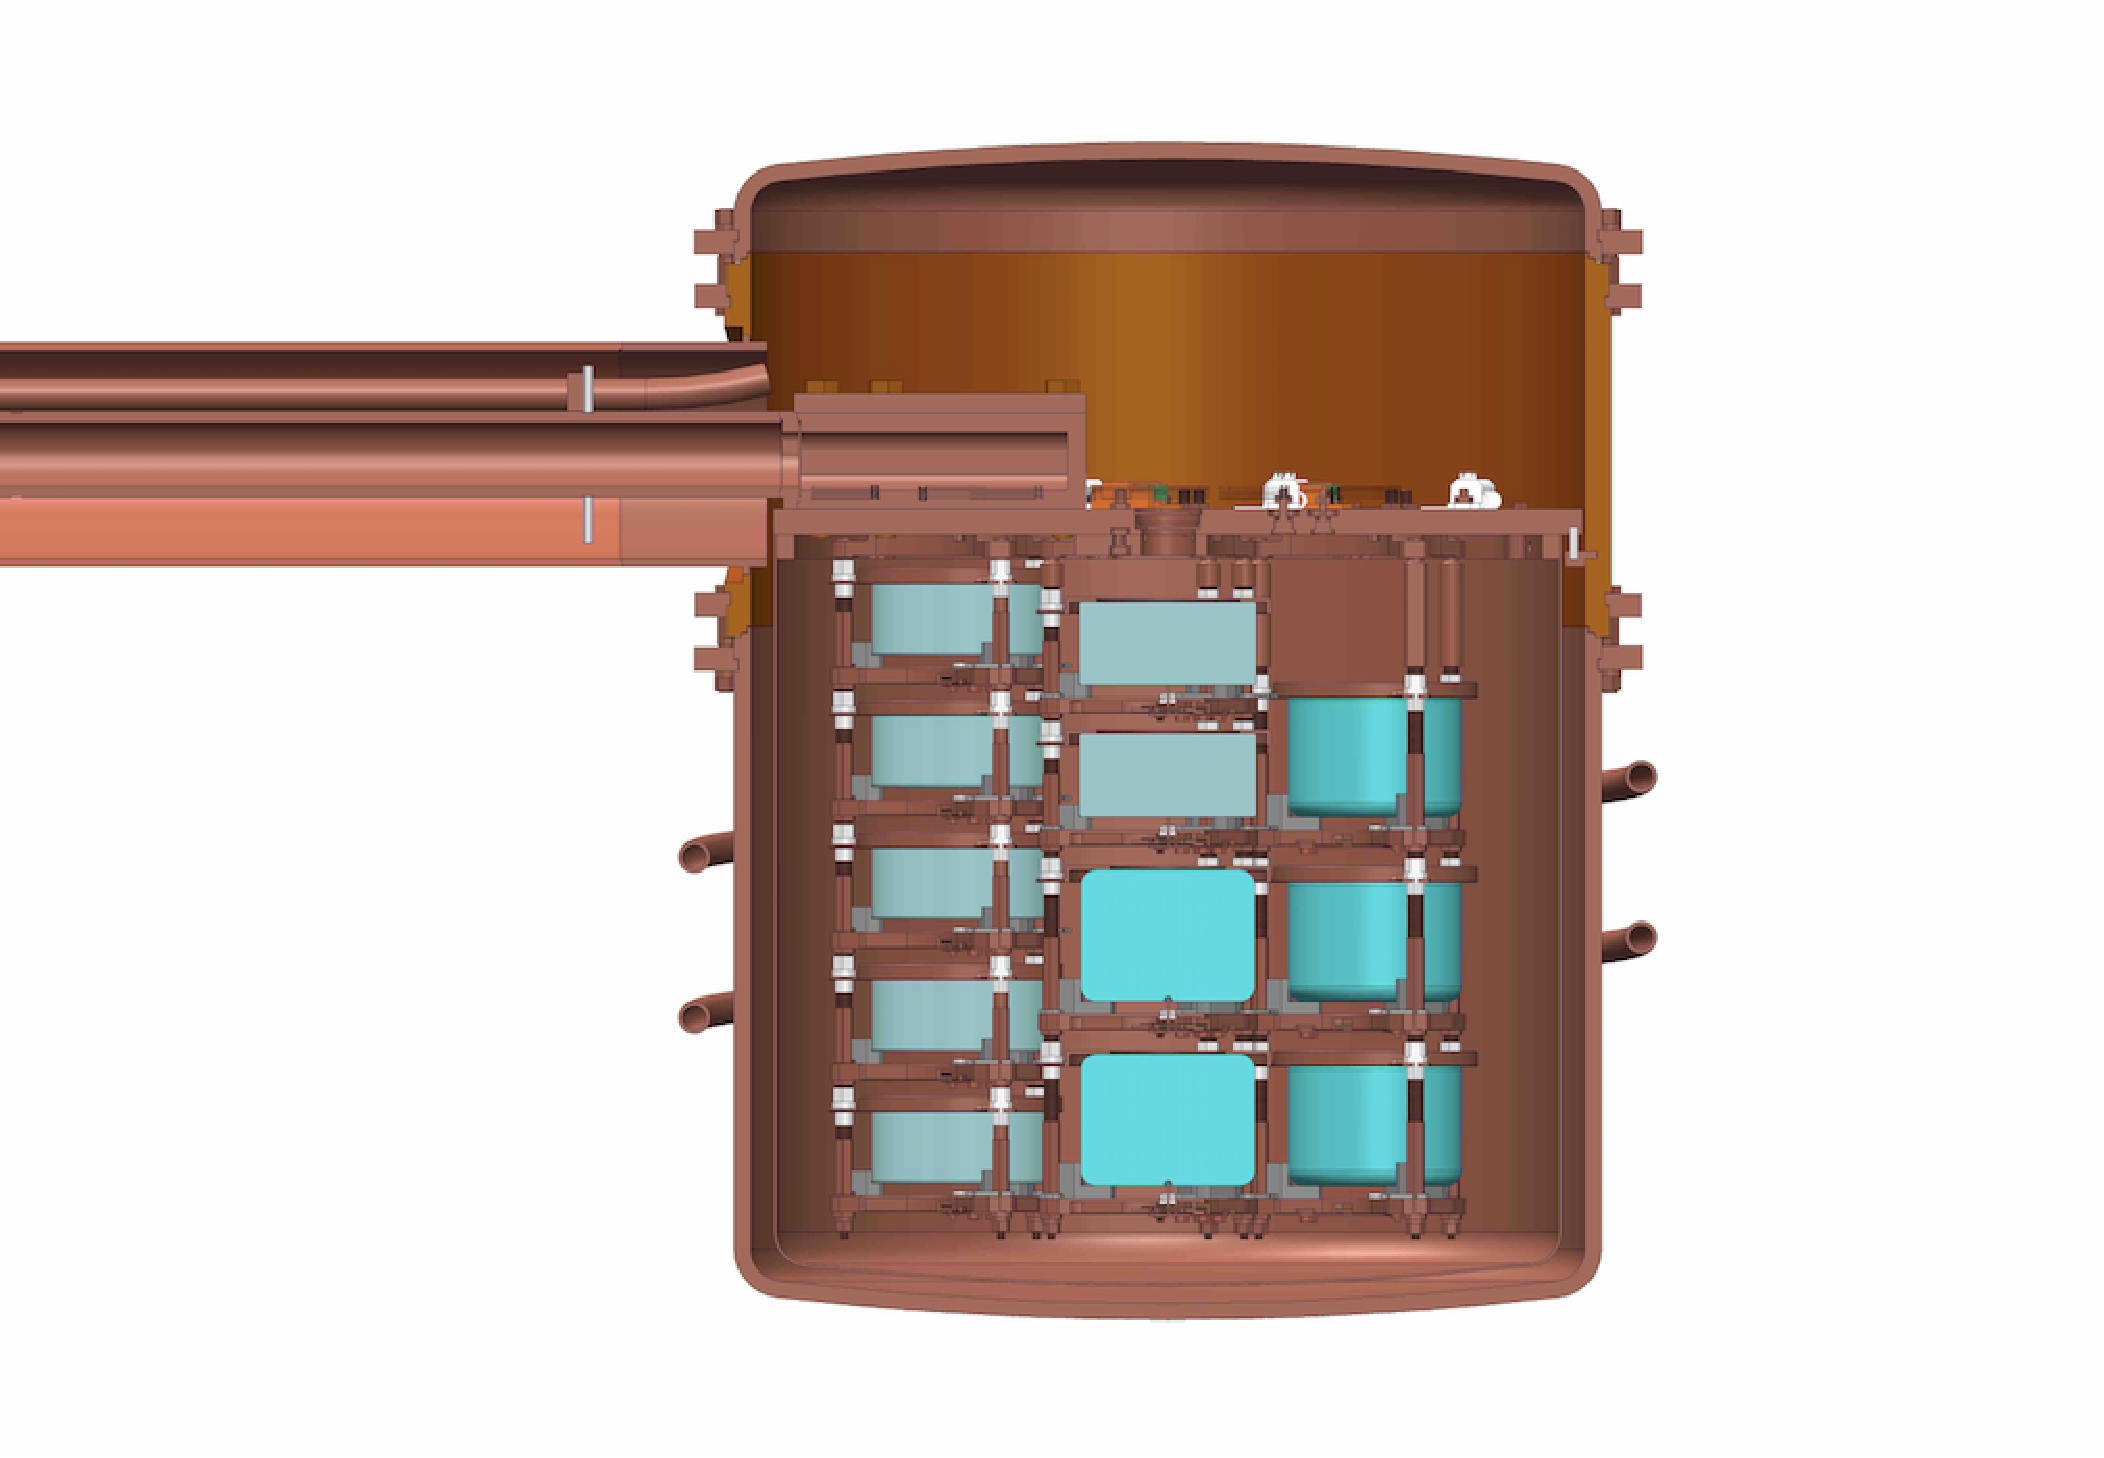
\includegraphics[width=0.7\textwidth]{/Users/cbartram/Downloads/example_diss/1_introduction/figures/mjd_cryostat.pdf}
\caption[%
\textsc{Majorana Demonstrator} cryostat drawing
]{%
Drawing of a \textsc{Majorana Demonstrator} cryostat. Strings of germanium crystals (turquoise) hang from the cryostat cold plate.
\label{fig:mjd_cryostat}} 
\end{figure}
% ------------  figure end 

